\section{The Evolution of the Neutral Hydrogen Fraction} % (fold)
\label{sec:the_evolution_of_the_neutral_hydrogen_fraction}
(Rahim)

	In order to place redshift limits on the epoch of reionization, the neutral hydrogen fraction will be calculated from the data procured. The optical depth will first be calculated using equation~(\ref{eq:optical_depth}) where the measured continuum flux can be compared to flux from an identical part of the spectrum of a lower redshift galaxy where the Gunn-Peterson trough is not visible. This can be done as the emitted spectra of Lyman break galaxies are very similar to that of much closer galaxies.

	The neutral hydrogen fraction can then be calculated via equation~(\ref{eq:gunn-peterson_tau}) and plotted as a function of redshift. Thus, when the neutral hydrogen fraction falls, a limit can be placed at a particular redshift for the end of the epoch of reionization. Figure~\ref{fig:Evolution_Xh1} shows an example of this where numerous methods are used to plot the evolution of the neutral hydrogen fraction\cite{Fanetal}.
	\begin{figure}[htbp]
		\centering
		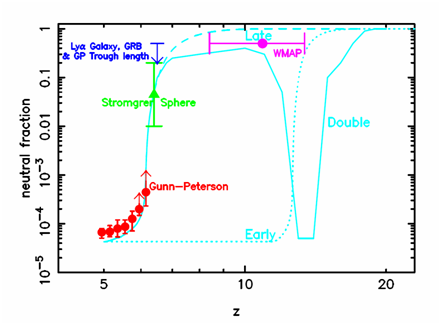
\includegraphics[width=0.5\textwidth]{../Images/Evolution_Xh1.png}
		\caption{The volume averaged fraction of neutral hydrogen in the IGM versus redshift. The fiducial model of late reionization is represented by the dashed line, an idealised model including double reionization is represented by the solid line and an early reionization model is represented by the dotted line.}\label{fig:Evolution_Xh1}
	\end{figure}

	With an initially large neutral hydrogen fraction, the radiation from early galaxies will start to ionise the neutral hydrogen causing the fraction to decrease indicating the start of the EoR. Towards the end of the EoR, at a certain redshift the spectra from galaxies will not show the Gunn-Peterson trough indicating a much lower fraction of neutral hydrogen. The redshift limit will therefore be the redshift at which production of the Gunn- Peterson trough ceases. Mapping the neutral hydrogen fraction should therefore place some rough limits on the start and end of the EoR.

	\subsection{Advantages and Disadvantages} % (fold)
	\label{sub:advantages_disadvantages}
		The main advantage of mapping the evolution of the neutral hydrogen fraction is that this can be done in conjunction with the dropout technique using the flux measured in that part of the observing strategy. However, a possible limitation of using the Gunn-Peterson absorption is that only a very small fraction of neutral hydrogen is required to produce complete Gunn-Peterson absorption. This means that the use of the Gunn-Peterson optical depth is more accurate towards the end of reionization where the IGM is already mostly ionised and the neutral hydrogen fraction is small. During the early part of reionization, it would be difficult to accurately measure the neutral hydrogen fraction as only a little is required to produce the Gunn-Peterson trough. However the redshift of the earliest galaxies in the universe will give the best idea of the redshift at which the EoR started as these galaxies contributed the first ionising radiation.
	% subsection advantages_disadvantages (end)
% section the_evolution_of_the_neutral_hydrogen_fraction (end)
